\documentclass{article}
\usepackage{tikz}
\usetikzlibrary{arrows}
\usepackage{booktabs, makecell, multirow}
\usepackage{siunitx}

% 2nd sections package
\usepackage{pgfplots}
\pgfplotsset{width=10cm,compat=1.9}
% We will externalize the figures
\usepgfplotslibrary{external}
\tikzexternalize

\begin{document}

\listoftables
\listoffigures

\vspace{5pt}
The table \ref{tab:1} and \ref{tab:2} are examples of referenced \LaTeX{} elements.
% The figure \ref{fig:3} is an example of referenced \LaTeX{} elements.

\section{Test table with tikz figure}

\begin{table}[htbp]
  \centering
  \caption{Table to test standalone in table.}
  \label{tab:1}
  \begin{tabular}{cccc}
    \toprule
    \textbf{include method} & \textbf{Figure 1} & \textbf{Figure 2} & \textbf{Figure 3} \\
    \midrule
    includegraphics & \includegraphics{figure1} & \includegraphics{figure2} & \includegraphics{figure3} \\
    includestandalone   & \includestandalone{figure1} & \includestandalone{figure2} & \includestandalone{figure3} \\
    includegraphics\\with\\scale   & \includegraphics[width=.2\linewidth] {figure1} & \includegraphics{figure2} & \includegraphics{figure3} \\
  \end{tabular}
\end{table}

test 


\begin{table}[htb]
  \caption{Another example of table with standalone}
  \label{tab:2}
  \centering
  \setcellgapes{3pt}
  \makegapedcells

  \begin{tabular}{cc *{4}{S[table-format=-2.2]}}
      \toprule
  Graph & Situation & {EV.diff.} & {Real.diff.} & {Best response} & {\# of obs.} \\
    \midrule
   \multirowcell{2}{
     \includegraphics{figure1}
     }
      &   1 (3) $\rightarrow$ 2   & 4     & 3.7  & 0.854  & 151       \\
      &   2 $\rightarrow$ 1 (3)   & -12   & -12  & 0.948  & 77        \\
      \cmidrule{2-6}
      \includegraphics{figure2}
      & 2 (3) $\rightarrow$ 1     &  4    & 2.67 & 0.24   & 25        \\
      \cmidrule{2-6}
   \multirowcell{6}{
     \includegraphics{figure3}
  }
      & 2 $\rightarrow$ 1         & -1.33 & 0.8   & 0.39  & 41        \\
      & 3 (4) $\rightarrow$ 1     & 4     & 4.17  & 0.889 & 27        \\
      & 3 (4) $\rightarrow$ 4 (3) & -4.7  & -6.33 & 0.676 & 37        \\
      & 1 $\rightarrow$ 3 (4)     & 4     & 4.25  & 0.5   & 32        \\
      & 1 $\rightarrow$ 2         & -12   & -12   & 1     & 13        \\
    \bottomrule
  \end{tabular}
\end{table}

\section{Tikz examples}
\subsection{Basic examples}
First example is 2D and 3D math expressions plotted side-by-side.

%Here begins the 2D plot
\begin{tikzpicture}
\begin{axis}
\addplot[color=red]{exp(x)};
\end{axis}
\end{tikzpicture}
%Here ends the 2D plot
\hskip 5pt
%Here begins the 3D plot
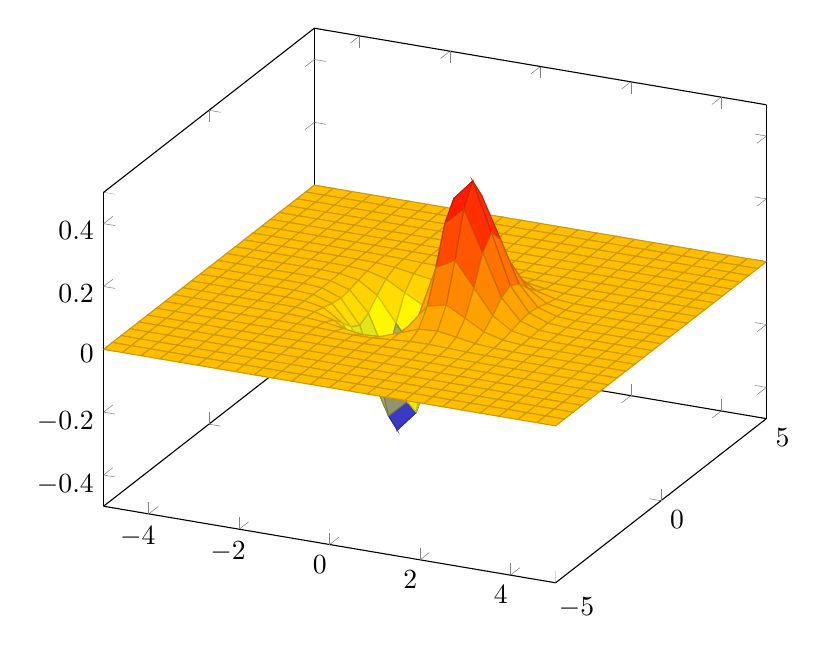
\begin{tikzpicture}
\begin{axis}
\addplot3[
    surf,
]
{exp(-x^2-y^2)*x};
\end{axis}
\end{tikzpicture}
%Here ends the 3D plot

\subsection{2D plot}
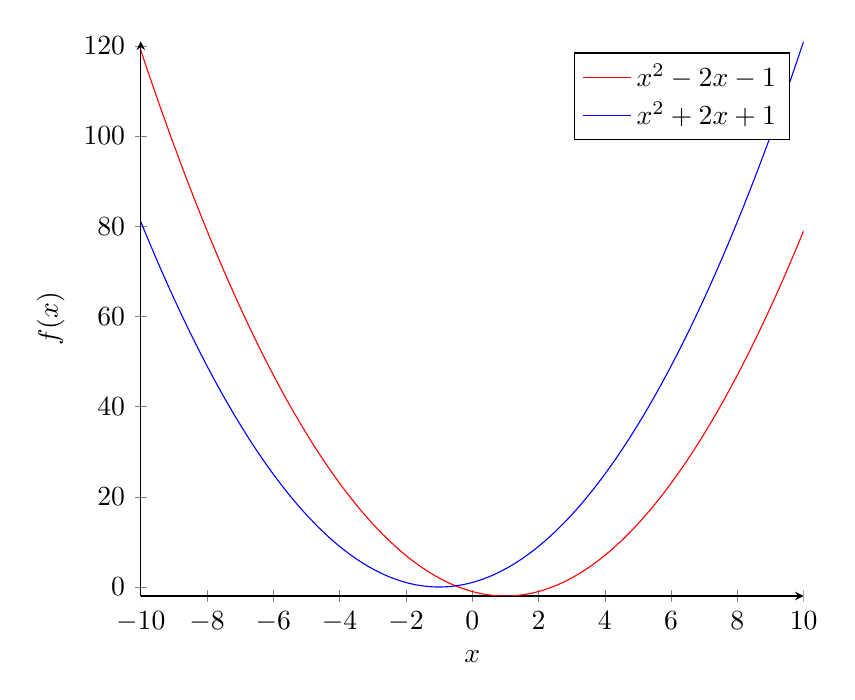
\begin{tikzpicture}
\begin{axis}[
    axis lines = left,
    xlabel = \(x\),
    ylabel = {\(f(x)\)},
]
%Below the red parabola is defined
\addplot [
    domain=-10:10, 
    samples=100, 
    color=red,
]
{x^2 - 2*x - 1};
\addlegendentry{\(x^2 - 2x - 1\)}
%Here the blue parabola is defined
\addplot [
    domain=-10:10, 
    samples=100, 
    color=blue,
    ]
    {x^2 + 2*x + 1};
\addlegendentry{\(x^2 + 2x + 1\)}

\end{axis}
\end{tikzpicture}

\subsection{Plotting from data}
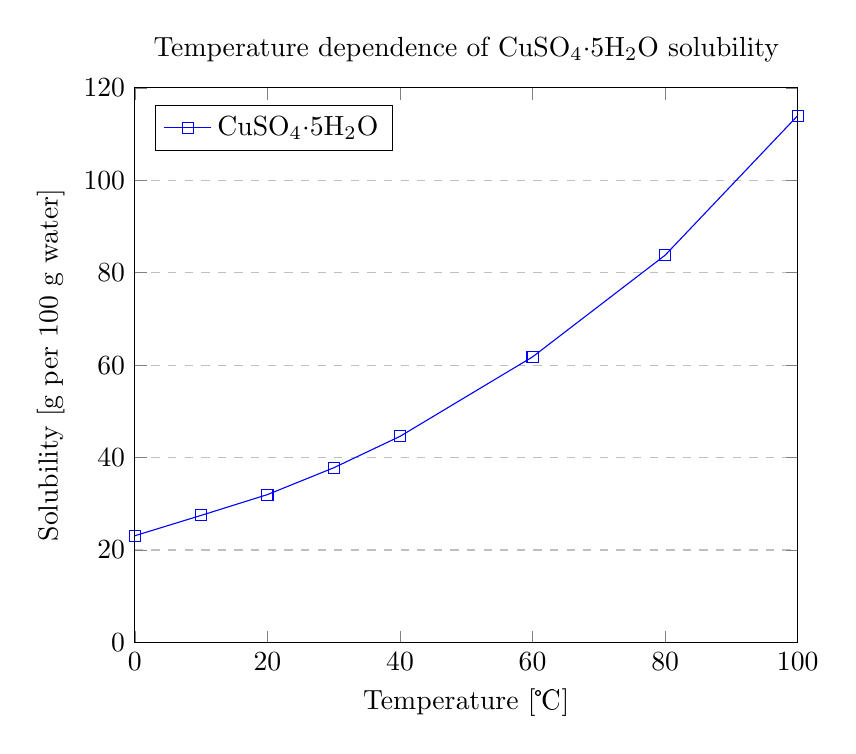
\begin{tikzpicture}
\begin{axis}[
    title={Temperature dependence of CuSO\(_4\cdot\)5H\(_2\)O solubility},
    xlabel={Temperature [\textcelsius]},
    ylabel={Solubility [g per 100 g water]},
    xmin=0, xmax=100,
    ymin=0, ymax=120,
    xtick={0,20,40,60,80,100},
    ytick={0,20,40,60,80,100,120},
    legend pos=north west,
    ymajorgrids=true,
    grid style=dashed,
]

\addplot[
    color=blue,
    mark=square,
    ]
    coordinates {
    (0,23.1)(10,27.5)(20,32)(30,37.8)(40,44.6)(60,61.8)(80,83.8)(100,114)
    };
    \legend{CuSO\(_4\cdot\)5H\(_2\)O}
    
\end{axis}
\end{tikzpicture}

\subsection{3D Plots with math expressions}
\begin{figure}
\centering
  \caption{Example of a parametric plot} \label{fig:3}
  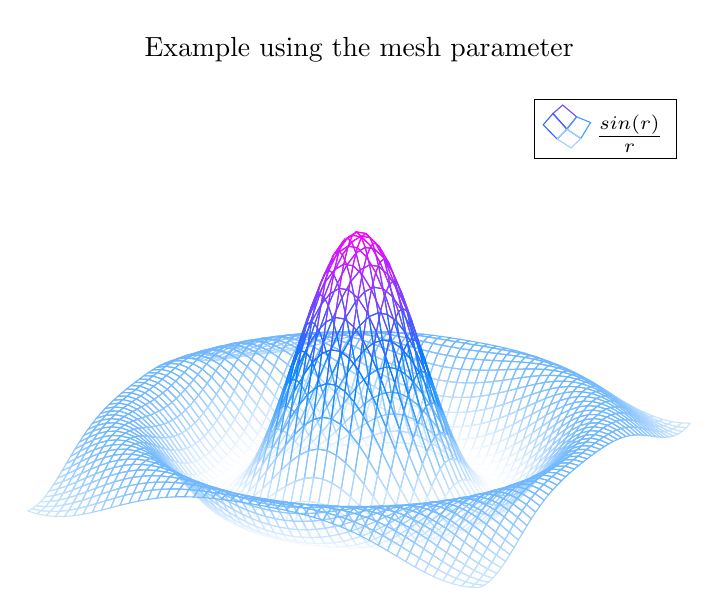
\begin{tikzpicture}
      \begin{axis}[
          title=Example using the mesh parameter,
          hide axis,
          colormap/cool,
      ]
      \addplot3[
          mesh,
          samples=50,
          domain=-8:8,
      ]
      {sin(deg(sqrt(x^2+y^2)))/sqrt(x^2+y^2)};
      \addlegendentry{\(\frac{sin(r)}{r}\)}
      \end{axis}
  \end{tikzpicture}
\end{figure}

\subsection{Table}
test
\begin{table*}[] \centering
%\ra{1.3}
\begin{small}
\begin{tabular}{@{}lllrrr@{}}\toprule
\textbf{Rank} & \textbf{Lead Arranger} & \textbf{Number of Deals} & \textbf{Dollar Amount} & \textbf{Market Share} & \textbf{Equator Principles Adoption}\\ \midrule
\textbf{1} & State Bank of India & 52 & \$21,631.6 & 10.1\% & NA\\ \hdashline
\textbf{2} & Mitsubishi UFJ Financial & 88 & 9,486.1 & 4.4 & Dec 2005\\ \hdashline
\textbf{3} & Sumitomo Mitsui & 71 & 8,188.1 & 3.8 & Jan 2006\\ \hdashline
\textbf{4} & Credit Agrocole & 60 & 6,506.4 & 3.1 & Jun 2005\\ \hdashline
\textbf{5} & Mizuho Financial & 55 & 5,797.5 & 2.7 & Oct 2003\\ \hdashline
\textbf{6} & Soci\'{e}t\'{e} Generale & 55 & 5,760.5 & 2.7 & Sep 2007\\ \hdashline
\textbf{7} & BNP Paribas & 55 & 5,390.8 & 2.5 & Oct 2008\\ \hdashline
\textbf{8} & Axis Bank & 18 & 5,216.9 & 2.4 & NA\\ \hdashline
\textbf{9} & IDBI Bank & 10 & 5,162.3 & 2.4 & NA\\ \hdashline
\textbf{10} & ING & 49 & 4,916.1 & 2.3 & Jun 2003\\ \midrule
 & Others & 102 & 135,430.4 & 63.6 & \\ \midrule
 & Total Market & 615 & \$213,486.7 & 100\% & \\
\bottomrule
\end{tabular}
\end{small}
\caption{Global project bank facility lead arrangers \emph{(Finnerty, 2013)}}
\end{table*}

\end{document}
